\section{Experiment Results}
\label{sec-exp}

To evaluate the accuracy of our hot-spot communication predictions and
the performance implications of our manually applied optimizations to
better overlap computation with communication, we applied our approach
to model and optimize 7 MPI applications from the NAS NPB~\cite{npb}
on two clusters shown in Figure~\ref{tab:hw}.  The first Intel
platform is a large high-performance computing cluster with very fast
internode communication through InfiniBand.  The second platform is in
a small data center where the internode communication is through
relatively slow Ethernet.  Both clusters use MPICH 3.1.1~\cite{mpich2}
as the underlying MPI library.  Because our current analytical
performance model cannot estimate intranode MPI communication time, we
have allocated a single MPI process per node on both clusters.

\begin{table}
\caption{Experiment platforms}
\begin{center}
\begin{tabular}{c|c c}
\hline
Server & Intel & HP ProLiant BL460c Gen6 \\
\hline
          &  Intel Xeon & Intel Xeon \\
Instruction set  &  x86 & x64 \\
Frequency &  2.6 GHz & 3.2 GHz \\
Compiler  &  ICC/Ifort 13.1 & GCC/Gfortran 4.4.7 \\
Network   &  InfiniBand Qlogic QDR & 1 Gbps Ethernet \\
Total nodes &  301 & 24 on 3 racks\\
Maximum memory &  64 GB & 48 GB \\
\hline
\hline
\end{tabular}
\end{center}
\label{tab:hw}
\end{table}

For each MPI application, we first used our extended SKOPE performance
modeling framework to find the most time-consuming MPI communication
in the application.  Then, we manually applied the
computation-communication optimization to the enclosing loop
surrounding the identified communications.  We measured the
performance improvements from the optimizations using input data
provided by the NPB benchmarks and using a range of 2 to 9 nodes for
each application.  Besides using the built-in timers within the NPB
applications to collect their overall performance, we manually
instrumented the source code of the applications to report the
performance of individual communications.


\subsection{Accuracy of Hot Communication Prediction}

To evaluate the accuracy of our modeling of MPI communications, we
compared the set of communication hot spots selected using our model
with those found by profiling the NPB applications, using class B
input on 4 nodes.  The different hot-spot selection for the NPB
applications are shown in Table~\ref{tab:npb:hot}.  When selecting the
top time-consuming MPI communications, we required that their overall
time be at least 80\% of the application's overall communication time.
In this case, our predictive modeling selected the same set of hot
communications as found using application profiling.  When asked to
select a given number of the most time-consuming communications,
however, the output by our predictive modeling differs by at most 2
selections compared with using profiling, for the NAS LU benchmark.
Here the most time-consuming communications are pairs of
sends/receives at four symmetric directions, which were estimated to
take the same time by our predictive modeling.  However, their actual
runtime collected through profiling differ by 37\%, because the
execution of the processes is unbalanced, resulting in extra wait time
to synchronize the corresponding MPI\_Send/MPI\_Recv operations.
Figure~\ref{fig:model:ft:B} compares our projected communication time
with the actual measured time for NAS FT, using two and four
processors.  Here in spite of the small error rates in projecting the
absolute values of the communication time, our modeling framework was
able to accurately capture the relative importances of the various
communication operations.

\begin{figure}
{\scriptsize
\begin{subfigure}{.48\textwidth}
\centering
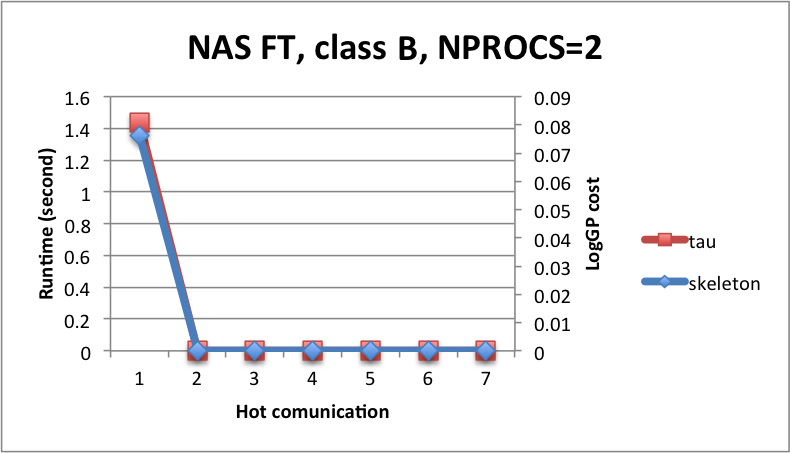
\includegraphics[width=.9\textwidth]{fig/blues/ft_B_2_model.png}
\caption{Communication on 2 nodes}
\label{fig:model:ft:B:2}
\end{subfigure}
\begin{subfigure}{.48\textwidth}
\centering
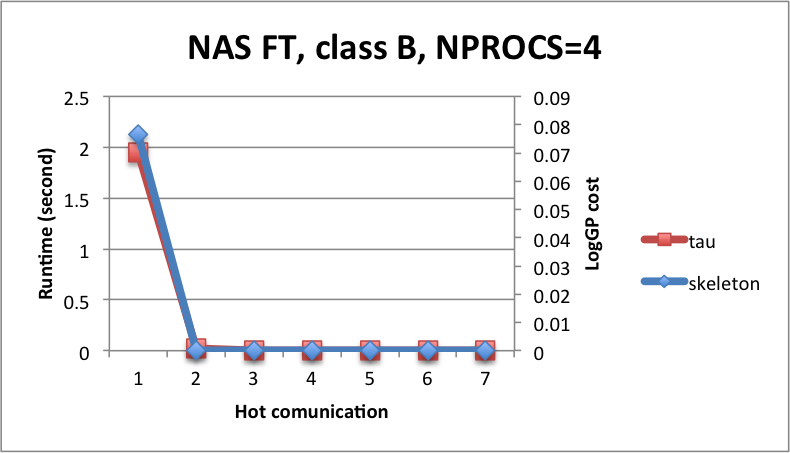
\includegraphics[width=.9\textwidth]{fig/blues/ft_B_4_model.png}
\caption{Communication on 4 nodes}
\label{fig::modelft:B:4}
\end{subfigure}
\caption{Profiled runtime and modeled cost of NAS FT with middle-sized input (B) on x86 cluster}
\label{fig:model:ft:B}
}
\end{figure}

\begin{table}
\caption{Differences between the projected hot-spot selection and the
  measured hot-spot selection based on profiling with 80\% threshold
  for class B data on 4 nodes. Zero means the set of $N$ hot spots
  equals the top $N$ hot spots.
}
\begin{center}
\begin{tabular}{c|r|r|r|r|r|r|r|r}
\hline
&\multicolumn{7}{c}{Selected number of hot MPI communications}\\
        & 1 & 2 & 3 & 4 & 5 & 6 & 7 & 8 \\
\hline
FT      & 0 &   &   &   &   &   &   &   \\  % 1:MPI_Alltoall, 99%
IS      & 0 & 0 &   &   &   &   &   &   \\  % 1:MPI_Alltoallv = 3.494, MPI_Allreduce = 1.279
CG      & 0 &   &   &   &   &   &   &   \\  % 1:MPI_Send 6,383, 2:MPI_Irecv
LU      & 0 & 1 & 2 & 2 & 1 & 1 & 0 & 0 \\  % MPI_Send
MG      & 1 & 1 & 0 & 1 & 1 & 0 &   &   \\  % MPI_Send
\hline
\hline
\end{tabular}
\end{center}
\label{tab:npb:hot}
\end{table}


\subsection{Impact of Optimizations}

\begin{figure}
{\scriptsize
\centering
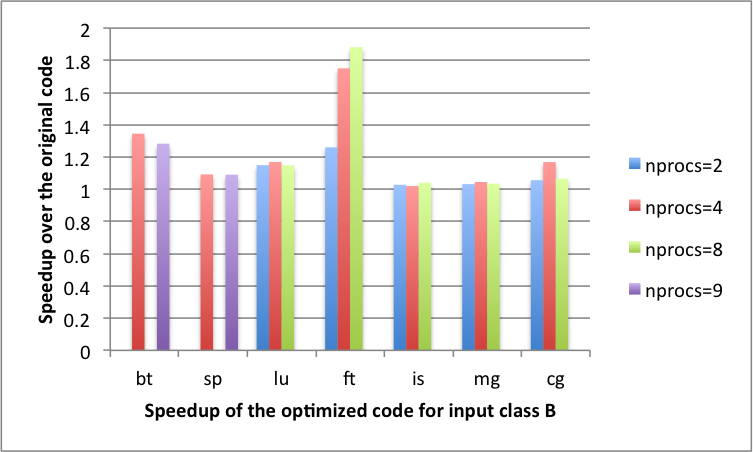
\includegraphics[width=.48\textwidth]{fig/blues/npb_blues_B.png}
\caption{Optimization speedups on the InfiniBand cluster.}
\label{fig:npb:x86}
}
\end{figure}
\begin{figure}
{\scriptsize
\centering
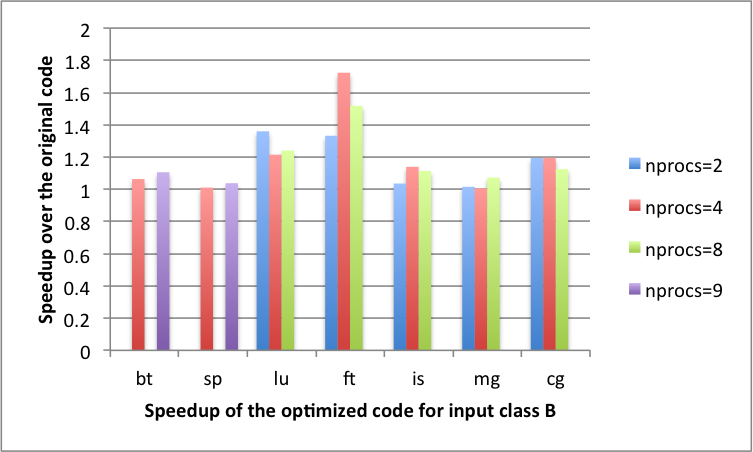
\includegraphics[width=.48\textwidth]{fig/disco/npb_disco_B.png}
\caption{Optimization speedups on the Ethernet cluster.}
\label{fig:npb:x64}
}
\end{figure}

Figures~\ref{fig:npb:x86} and \ref{fig:npb:x64} show the speedups we
attained by enabling better computation-communication overlapping for
the NPB applications.  In particular, for each benchmark, the
performance of the original application and the optimized code is
measured by using input class B on 2, 4, 8, and 9 nodes, with one MPI
process bound to each node, with the exception of NAS BT and SP, which
require the number of processes to be a multiple of 3 and so are
configured to run on 3 and 9 nodes only.  The overall elapsed time of
each application is measured by using NPB's built-in timer, which
reports the elapsed time of multiple iterations with the exclusion of
the initialization time.

Among all the NPB applications, FT and IS are the only benchmarks that
use {\em alltoall} collectives as the main communication operation;
the other benchmarks mostly use point-to-point send/receives.  Our
optimization attained 3--88\% speedup for all applications.  The
maximum 88\% performance improvement is observed with the NAS FT
benchmark, which uses a time-consuming $MPI\_Alltoall$ operation,
enclosed inside the outermost loop of the application, to exchange a
large amount of data.  The lowest speedup (3\%) is observed with NAS
MG, which does not have sufficient local computation in the
surrounding loop of the MPI communication to overlap with
communication. \todo {I think we need to discuss more the difference
  between using the two different platforms}
